% !TEX root=/home/tavant/these/manuscript/src/manuscript.tex




\chapter{Particle-In-Cell simulations of Hall Effect Thrusters}
\label{ch-1}
Structure :

{\bf Particle in Cell simulations} 20 pages
\begin{zzz}
  
  1.1 The HET
  1.2 Elements of the 2D PIC-MCC simulations

  1.3 Numerical implementation

  1.4 R-theta simulation: hypotheses
  
  1.5 focus on  Dielectrics : Poisson equation 

  1.6 Axial convection model
  
  1.7 Conclusion
\end{zzz}
\inlinenote{Is missing a part of the HET physics. Like the Boeuf Tutorial. }
\inlinenote{Missing SEE }

The \ac{HET} has been studied since its first designs int he 1960's.
However, the physical processes the govern its behaviour stay ill-understood.
For most of them, as the electron cross field mobility or the plasma-surface interactions, kinetic informations are needed.


The next section present the basics of the \ac{PIC} - \ac{MCC} simulations, and the simulations code \LPPic that is develop at \ac{LPP}.


\inlinenote{add SEE models, discussions concerning the choice we did, a.s.o.}
 
% !TEX root=/home/tavant/these/manuscript/src/manuscript.tex


% !TEX root=/home/tavant/these/manuscript/src/manuscript.tex

\section{Elements of the 2D PIC-MCC simulations}
  \label{sec-elements}
  \subsection{Principe of the PIC simulations}

    The \ac{PIC} simulation models particles moving freely on a grid.
    The grid is used to compute the electric field, in the electrostatic approximation by solving the Poisson equation

    \begin{equation}
      \label{eq-poisson}
      \Delta \phi = - \frac{\rho}{\epsilon_0}
    \end{equation}

    where $\phi$ is the electric potential, $\rho$ is the charge density, and $\epsilon_0$ the vacuum permittivity.
    If the electrostatic approximation is not correct, one need to solve the Maxwell equations.

    The particles move following the Lorenz forces
    \begin{equation}
      \label{eq-Lor}
      m \vec{a} = q \vect{E} + q \vec{v} \times \vec{B}
    \end{equation}
    with $m$ and $q$ the particle mass and electric charge respectively.
    The numerical particles followed in the simulations correspond to $q_f$ physical particles, with
    \begin{equation}
      q_f = \frac{n V}{\Npc}
    \end{equation}
    with $n$ the particle density, $V$ the volume of a cell, and $\Npc$ the number of numerical particle in a cell.
    A large enough number of particle is needed in order to obtain physical results.
    Indeed, insufficient number of particles leads to numerical heating \cite{ueda1994}.
    Usually, a minimum of 100 particles per cell are used, but recent results seem to encourage to use more particle \cite{janhunen2018}.

  \subsection{Monte Carlo collisions}

    In \ac{PIC} simulations, collisions between charged and neutral particles can be modeled by binary collision, but this approach is computationally costly.
    Instead, a Monte-Carlo algorithm can be used \cite{vahedi1995}.
    This approach is very efficient, and allow scattering, momentum transfer and ionization to be consistently modeled.
    The propellant used in \ac{HET} usually is \ac{Xe}, even if the recent constellation Starlink uses \ac{Kr}.
    The cross sections used for modeling \ac{Xe} or other gases collisions are taken from the {\sc LXCat} database project \cite{LXCat_web}.
    Except if otherwise stated, the elastic, inelastic scattering and ionization reactions listed in \cref{tab-reactXe} are used.
    The cross section values are summarised in \cref{fig-xexsection}.

    \begin{table}[hbtp]
      \ra{1.3}
      \centering
      \caption{Reactions for xenon used in the PIC simulations}
      \label{tab-reactXe}
      \begin{tabular}{@{}lll@{}}  \toprule
        Reaction & Threshold & Reference\\ \midrule
        {\it Elastic scattering} & &\\
        e + Xe = e + Xe   & --   & \cite{Lxcat_Xe,Lxcat_Xe2} \\
        {\it Excitation} & &\\
        e + Xe = e + Xe$^*$   & 8.315eV   & \cite{Lxcat_Xe,Lxcat_Xe2} \\
        e + Xe = e + Xe$^*$   & 9.447eV   & \cite{Lxcat_Xe,Lxcat_Xe2} \\
        e + Xe = e + Xe$^*$   & 9.917eV   & \cite{Lxcat_Xe,Lxcat_Xe2} \\
        e + Xe = e + Xe$^*$   & 11.7eV    & \cite{Lxcat_Xe,Lxcat_Xe2} \\
        {\it Ionization} & &\\
        e + Xe = e + Xe$^+$   & 8.315eV   & \cite{Lxcat_Xe,Lxcat_Xe2} \\
        \bottomrule
      \end{tabular}
    \end{table}



    \begin{figure}[hbtp]
      \centering
      \includegraphics[width=\defaultwidth]{figure/xenon_cross_section.pdf}
      \caption{Cross section values used in the Monte Carlo procedure \cite{Lxcat_Xe,Lxcat_Xe2}.}
      \label{fig-xexsection}
    \end{figure}


\section{Numerical implementation of the Particle in cell simulation}

  \LPPic is an explicit electrostatic \ac{PIC}-\ac{MCC} simulation code.
  Every time-steps, the simulation loop presented in \cref{fig-picloop} is computed.
  The different steps constituting the PIC-loop are described in the next subsections.
  \begin{figure}[hbtp]
    \centering
    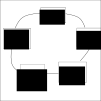
\includegraphics{picloop.png}
    \caption{\ac{PIC}-\ac{MCC} loop executed every time steps.}
    \label{fig-picloop}
  \end{figure}

  \subsection{Data used}
    In the \ac{PIC} simulations, there are two kind of data used\string:
    \begin{itemize}
      \item Particles (electron, ions, neutral can be followed as well but not in \LPPic)
      \item Mesh, also named fields (densities, electric and magnetic fields, and so on)
    \end{itemize}

    \paragraph{Particles\\}
    For each particles, are known its position $\vec{x}$ and its velocity $\vec{v}$.
    In most \ac{PIC}-\ac{MCC} simulations, the 3 directions of the velocity vector are followed in order to in order to take into account scattering.
    It is abbreviated as \acs{3V}.
    
    \paragraph{Fields\\}
    The fields are defined at the center of each cell of the mesh.
    The charge density $\rho$ is computed by depositing the particle on the mesh, using the Cloud-in-cell model \cite{birdsall1991}.
    The electric field at the position of the particle is also obtain by bi-linear interpolation.
    The mesh dimension defines the dimension of the simulation.
    It is usual to find \acs{1D}\acs{3V} or \acs{2D}\acs{3V} \ac{PIC} simulations, for particles with 3 directions on the velocity but 1 (or 2) dimensions in space.

    \subsection{Particle pusher}
    The interaction of the movement equation \cref{eq-Lor} is different for magnetized and non-magnetized particles.

    For non-magnetized particles, we use the leapfrog scheme \cite{birdsall1991}
    \begin{align}\label{eq-leapfrog}
      \vect{v}^t &= \vect{v}^{t-1} + \frac{q}{m} \vect{E} \dt, \\
      \vect{x}^t &= \vect{x}^{t-1} + \vect{v}^t \dt,
    \end{align}
    with the superscript $t$ designing the time step, $q$ and $m$ the particle electric charge and mass, $\vect{E}$ the electric field at the particle position, and \dt the time step duration.

    It is important to note that the leapfrog induces a shift of $\frac{\dt}{2}$ between the position and the velocity, as illustrated in \cref{fig-leapfrog}.
    \begin{figure}[hbtp]
      \centering
      \includegraphics[width=\defaultwidth]{leapfrog.png}
      \caption{Illustration of the shift between the particle velocity and position.}
      \label{fig-leapfrog}
    \end{figure}
    This shift can leads to erroneous diagnostics when computing moments of the particles distribution.
    For instance, the mean velocity of an ensemble of $N$ particle at the instant $t$ is computed as\string:
    \begin{equation} \label{eq-meanv}
      \mean{\vect{v}}^t = \frac{1}{N} \sum_i^N \lp \vect{v_i}^t + \frac{q}{m} \vect{E_i} \frac{\dt}{2} \rp.
    \end{equation}
    Other moments like the mean energy or heat flux follow the same correction.
    We can see that the error between $\mean{\vect{v}}$ defined above and
    $$ \tilde{\vect{v}} = \frac{1}{N} \sum_i^N  \vect{v_i}^t $$
    is
    $$ \mean{\vect{v}} - \tilde{\vect{v}} =\frac{q \dt}{2 m}  \frac{1}{N}  \sum_i^N  \vect{E_i} .$$
    Hence, the error in the diagnostic is larger in the region of large electric field (as in the sheaths).

    \paragraph{Magnetized particles}
    For magnetized particles, we use a modification of the leapfrog algorithm proposed by Boris \cite{boris1970}.
    It correspond to an operator splitting between the electrostatic acceleration and the magnetic rotation.
    This splitting is describe below\string:

    \begin{enumerate}
      \item accelerate the particle during $\frac{\dt}{2}$ \string: $\vect{v}^{t-\frac{\dt}{2}} = \vect{v}^{t-1} + \frac{q}{m} \vect{E} \frac{\dt}{2}$
      \item rotate the particle velocity with the magnetic field
      \item accelerate the particle during $\frac{\dt}{2}$ \string: $\vect{v}^t = \vect{v}^{t-\frac{\dt}{2}} + \frac{q}{m} \vect{E} \frac{\dt}{2}$
    \end{enumerate}


  \subsection{Poisson equation solver}
  \label{subsec-poissonintro}

    The Poisson equation \cref{eq-poisson} is an elliptic equation.
    We can directly discretize the differential operator by finite volume on the cell mesh.
    The formal discretization is develop in \cref{sec-diel}, but a short summary is given here.

    In \ac{1D}, the obtained linear system is tridiagnonal.
    It can be solve directly using {\sc Thomas} algorithm, which simply stores the Gauss elimination's coefficient.
    In \ac{2D}, the linear system is pentadiagonal.
    A direct solver, like the $LU$ decomposition, would require a large amount a memory to store the factorisation matrices.
    On the other hand, as the time step is usually small in \ac{PIC} simulation, we expect the plasma potential $\phi$ not to change rapidly.
    Hence, an iterative solver using the previous solution as initial guess seems more reasonable fro both the memory storage and the computational time.

    In practice, we uses {\sc Hypre}'s multigrid solver to solve Poisson equation in \ac{2D} in \LPPic.

% !TEX root=/home/tavant/these/manuscript/src/manuscript.tex

\section{Bidimentionnal simulation of an Hall Effect Thruster}


\subsection{The Hall effect Thruster }

The \ac{HET} is an electrostatic electrical propulsion system accelerating ions by the mean of an imposed voltage difference.

We can summarize its composition by four parts:
\begin{enumerate}
  \item The annular chamber.
  \item The injecting anode
  \item The cathode
  \item The magnetic circuit
\end{enumerate}

\paragraph{The chamber} has an annular shape.
It is open closed at the anode side, and kept open at the other side.
The walls are usually constituted by a ceramic, usually \ac{BNSiO2}.
The material needs to be resistant to erosion by ion impact sputtering.
But changing the material is also known to affects the discharge behaviour.
The usually supposed phenomena for this impact is the secondary electron emission yield that is a function of the material nature.


\paragraph{The anode} is at the bottom of the chamber.
The anode voltage is imposed to a few hundred volts.
Usually, the neutral gas injection is made by the anode itself.
The mass flow rate is of the order of a flew mg/s.

\paragraph{The cathode} is outside of the chamber.
It is grounded, and injects electrons for two reasons:
\begin{itemize}
  \item most of the electrons ($\sim 90 \%$) are used to neutralize the ion flux, for both allowing the ions to leave the thruster and avoid charging of the spacecraft.
  \item some of the electrons are attracted by the anode, hence entering the chamber and allowing the plasma discharge and switch and remain on.
\end{itemize}

% !TEX root=/home/tavant/these/manuscript/src/manuscript.tex

\section{Dielectrics boundary condition}
  \label{sec-diel}

  \Cref{fig-2dschemat} shows the simulation of the radial-azimuthal domain with metallic grounded walls.
  \Cref{fig-2D} illustrates the configuration in the radial-azimuthal planehighlighting the more realistic radial boundary conditions.
  The plasma is bounded in the radial direction by dielectric layers isolating the magnetic circuit.
  The magnetic circuit can be considered electrically grounded.

  The particles are absorbed when touching the dielectric wall, and we suppose an infinite residence time.
  Hence, we obtain a surface charge $\sigma$ at a time $t$ with
  \begin{equation} \label{eq-sigmaintegrate}
    \sigma(t) = e \int_0^t (J_i - J_e) dt
  \end{equation}
  with $J_i$ and $J_e$ the ion and electron flux respectively and $e$ is the elementary charge and supposing that there is no surface charge at the interface at the beginning.

  \begin{figure}[hbtp]
    \centering
    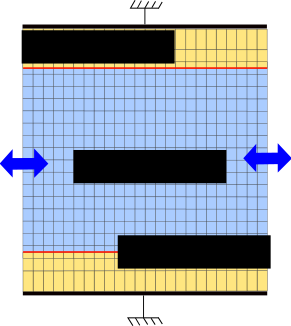
\includegraphics[width=\defaultwidth]{2D_diel_Rtheta}
    \caption{Schematic representation of the dielectric layers between the plasma in the \ac{2D} radial-azimuthal plan. Are present the dielectric in yellow, the plasma in blue, the surface charges in red and the grounded magnetic circuit in black.}
    \label{fig-2D}
  \end{figure}


  A common approach is to suppose that the electric field inside the dielectric is zero \citep{taccogna2019}. 
  Using Gauss theorem, we obtain a Neumann boundary condition at the plasma-wall interface for the potential
  \begin{equation} \label{eq-gauss}
    \norm{\partial_r \phi} = \frac{\norm{\sigma}}{\epsilon_0}
  \end{equation}
  with $\sigma$ the surface charge and $\epsilon_0$ the vacuum permittivity.
  However, the electric field in a dielectric material is not zero, but depends on the global system.
  Hence, in order to model correctly the dielectric wall of the \ac{HET}, we choose to include the whole dielectric layers inside of the simulation domain.

  In this section, we derive the discretization of the Poisson equation with non-uniform permittivity in the \ac{2D} radial azimuthal plane using the finite volume approach.


  \subsection{Non-uniform mesh}

    In the dielectric layers, there is no particle nor charge.
    Hence, the numerical constraints on the cell size are not applicable, and the cell size can be increased.
    In order to reduce the cell size difference between two neighbouring cells, we use an exponential growth of the cell size in the radial direction.
    The cell size in the azimuthal direction $\dy$ is kept constant.
    The resulting non-uniform mesh can be seen in \cref{fig-2D}.


  \subsection{Poisson equation discretization}


  The dielectric permittivity is $\epsilon= \epsr \epsilon_0$ with $\epsr$ the relative permittivity of the dielectric.

  The Poisson equation with not-constant permittivity is
  \begin{equation} \label{eq-poissondiel}
    \grad \cdot \epsilon \grad \phi = \rho
  \end{equation}
  with $\rho$ the charge density.
  We note $\vect{D}=\epsilon \vect{E} = \epsilon \grad \phi$ the electric flux.

  \Cref{fig-decompo1} shows the Cartesian decomposition of the \ac{2D} domain.
  The cell $(i,j)$ has four direct neighbours\string:
  \begin{itemize}
    \item the east $E$ in $(i+1,j)$
    \item the west $W$ in $(i-1, j)$
    \item the north $N$ in $(i, j+1)$
    \item the south $S$ in $(i, j-1)$
  \end{itemize}
  The cell dimensions are $\dx_{i,j}$ and $\dy_{i,j}$, and $\V=\dx_{i,j} \dy_{i,j}$ is the cell volume.
  As the mesh is Cartesian, we have for a given $j$ $\dx_{i,j} = cst$ for all $i$. Hence, we note $\dx_{i,j} = d_i$ and $\dy_{i,j} = d_j$

  The boundaries are noted $S^s_{i,j}$ with $s=E,W,N$ or $S$.
  We can see that $S^W_{i,j}=S^E_{i-1,j}$, and the same goes for the other borders.
  We note $\C = S^E_{i,j} \cup S^W_{i,j} \cup S^N_{i,j} \cup S^S_{i,j}$ the cell surface boundary.
  The center of the cell is located in $i,j$ and the borders are located in $i\pm 1/2$ in the East-West direction and $j\pm 1/2$ in the North-Sourth direction.
  \begin{figure}[hbt]
    \centering
    \includegraphics[width=\defaultwidth]{discrect1.pdf}
    \caption{Illustration of the Cartesian decomposition of the \ac{2D} domain}
    \label{fig-decompo1}
  \end{figure}


  \subsection{Poisson equation discretization}

    We start by positioning the plasma-dielectric interface on the surface between two cells.
    This means that the permittivity $\epsilon = \epsilon_0 \epsr$ is  constant over a cell.
    In order to discretize the Poisson equation, we integrate \cref{eq-poissondiel} over the cell volume

    \begin{equation}
    \int_{\V} - \grad \cdot (\epsilon \grad \phi) dv= \int_{\V} \rho dv.
    \end{equation}
    Using Gauss-Ostrogradsky theorem, we obtain
    \begin{equation}
    \oint_{\C} ( - \epsilon \grad \phi) \cdot \vect{n} dS = Q_{tot} =  \V \bar{\rho},
    \end{equation}
    with $\vect{n}$ the normal vector directed outward, $Q_{tot}$ is the total charge of the cell and $\bar{\rho}$ is the mean value of $\rho$ in the cell.
    We can decompose the integration over the cell boundary with the four surfaces $S^s_{i,j}$ as
    \begin{equation}
      \label{eq-poissonsum}
    \oint_{\C} (-\epsilon \grad \phi) \cdot \vect{n} dS = \sum_{k\in(E,W,N,S)} S^k_{i,j} \vect{D}^k_{i,j} \cdot \vect{n}
    \end{equation}
    with $\vect{D}^k_{i,j}$ the flux through the surface $k$ of the cell $(i,j)$.


    \paragraph*{Electric flux \\}
    Let us define the electric flux through the East border  $\vect{D}^E_{i,j}$.
    We suppose there is no surface charges on $S^E$.
    We can hence write the electric flux as
    \begin{align} \label{eq-flux1}
      \vect{D}^E_{i,j} \cdot \vect{n} &= \epsilon_{i,j} E_{x, i+1/2,j}^-\\
                                      &= - \epsilon_{i,j} \frac{\phi_{i+1/2,j} - \phi_{i,j}}{d_i/2},
    \end{align}
    with an off-center discretization of the electric field.

    Using the Gauss's law without charges
    \begin{equation} \label{eq-gausslaw}
      \epsilon_{i,j}E_{x, i+1/2,j}^- - \epsilon_{i+1,j}E_{x, i+1/2,j}^+ =0,
    \end{equation}
    we have
    \begin{equation}
      \epsilon_{i,j} \frac{\phi_{i+1/2,j} - \phi_{i,j}}{d_i/2} = \epsilon_{i+1,j} \frac{\phi_{i+1,j} - \phi_{i+1/2,j}}{d_{i+1}/2}.
    \end{equation}
    Hence
    \begin{equation} \label{eq-phidemi1}
      \phi_{i+1/2,j} = \frac{\epsilon_{i,j} d_{i+1} \phi_{i,j} + \epsilon_{i+1,j} d_{i} \phi_{i+1,j} }{\epsilon_{i,j} d_{i+1} + \epsilon_{i+1,j} d_{i} },
    \end{equation}
    which corresponds to the usual discretization when $\epsilon$ and $d_i$ are both constant.
    Using \cref{eq-phidemi1} in \cref{eq-flux1} we obtain
    \begin{align}
      \label{eq-nosc}
    \vect{D}^E_{i,j} \cdot \vect{n} &=& 2\frac{\epsilon_{i,j}\epsilon_{i+1,j}}{\epsilon_{i,j}d_{i+1} + \epsilon_{i+1,j} d_i} (\phi_{i,j}-\phi_{i+1,j})
    &=& 2\epsilon_0 \frac{\epsr{i,j}\epsr{i+1,j}}{\epsr{i,j}d_{i+1} + \epsr{i+1,j} d_i} (\phi_{i,j}-\phi_{i+1,j})
    \end{align}

    We note $Q^E_{i,j} \equiv \frac{\epsilon_{i,j} \epsilon_{i+1,j}}{\epsilon_{i,j} d_{i+1} + \epsilon_{i+1,j} d_i}$.
    reproducing the same decomposition on the other borders, we obtain
    \begin{equation}
      \label{eq-descretPoisson1}
    S^E_{i,j} Q^E_{i,j} \phi_{i+1,j} + S^W_{i,j} Q^W_{i,j} \phi_{i-1,j} + S^N_{i,j} Q^N_{i,j} \phi_{i,j+1} + S^S_{i,j} Q^S_{i,j} \phi_{i,j-1} - Q^C_{i,j} \phi_{i,j} = - \V \bar{\rho_{i,j}}
    \end{equation}
    with
    \begin{center}
      $\begin{dcases}
     Q^E_{i,j} &= 2\frac{\epsilon_{i,j} \epsilon_{i+1,j}}{\epsilon_{i,j} d_{i+1} + \epsilon_{i+1,j} d_i} \\
     Q^W_{i,j} &= Q^E_{i-1,j} \\
     Q^N_{i,j} &= 2\frac{\epsilon_{i,j} \epsilon_{i,j+1}}{\epsilon_{i,j} d_{j+1} + \epsilon_{i,j+1} d_{j}}\\
     Q^S_{i,j} &= Q^N_{i-1,j} \\
     Q^C_{i,j} &= Q^E_{i,j}S^E_{i,j}+Q^W_{i,j}S^W_{i,j}+Q^N_{i,j}S^N_{i,j}+Q^S_{i,j}S^S_{i,j}
     \end{dcases}$
    \end{center}

    as well as $S^E_{i,j} = S^W_{i,j} =d_id_z, S^N_{i,j} = S^S_{i,j}= d_jd_z$ et $\V = d_jd_id_z$.
    We observe that the evolution of the relative permittivity and the cell size affects the coefficients to be used, but the system remains symmetric as we have $Q^S_{i,j} = Q^N_{i-1,j}$ and $ Q^W_{i,j} = Q^E_{i-1,j}$.
    
    A symmetric system is a linear system of equation $A \cdot X = B$  which matrix $A$ is equal to is transpose: $A = A^T$.
    It allows to reduce by a factor of two the memory needed to store the matrix.
    It also allows to use algorithm exploiting this aspect. For instance, the eigenvalues are real-valued, and the matrix factorisation only need to store one factor using Cholesky decomposition, which gives $A = L L^T$ with L an upper-triangular matrix. 

    \subsection{Including surfaces charges}
    Let's now considerer the presence of surface charges on the surface $S^E_{i,j}$.
    Gauss's law now reads
    \begin{equation} \label{eq-gausslawsc}
      -\epsilon_{i,j}E_{x, i+1/2,j}^- + \epsilon_{i+1,j}E_{x, i+1/2,j}^+ =\sigma^E,
    \end{equation}
    with $\sigma^E$ the surface charge on the surface.
    The surface charge is not taken into account when computing the total charge in a cell.
    Using the same discretization as before, we obtain
    \begin{equation}
    \epsilon_{i,j} \frac{\phi_{i+1/2,j} - \phi_{i,j}}{d_i/2} - \epsilon_{i+1,j} \frac{\phi_{i+1,j} - \phi_{i+1/2,j}}{d_{i+1}/2} = \sigma^E
    \end{equation}
    so that
    \begin{equation}
      \label{eq-phidemi}
    \phi_{i+1/2,j} = \frac{\epsilon_{i,j} d_{i+1} \phi_{i,j} + \epsilon_{i+1,j} d_{i} \phi_{i+1,j} }{\epsilon_{i,j} d_{i+1} + \epsilon_{i+1,j} d_{i} } + \frac{1}{2}\sigma^E \frac{d_i d_{i+1}}{\epsilon_{i,j} d_{i+1} + \epsilon_{i+1,j} d_{i}}
    \end{equation}
    hence
    \begin{align*}
    \vect{D}^E_{i,j} \cdot \vect{n} &= 2\frac{\epsilon_{i,j}\epsilon_{i+1,j}}{\epsilon_{i,j}d_{i+1} + \epsilon_{i+1,j} d_i} (\phi_{i,j}-\phi_{i+1,j}) - \sigma^E \frac{\epsilon_{i,j}d_{i+1}}{\epsilon_{i,j}d_{i+1}+\epsilon_{i+1,j}d_{i}}
    \end{align*}
    We obtain the same relation that \cref{eq-nosc} updated by $- \sigma^E \frac{\epsilon_{i,j}d_{i+1}}{\epsilon_{i,j}d_{i+1}+\epsilon_{i+1,j}d_{i}}$

    Hence, we finally obtain
    \begin{equation}
    S^E_{i,j} Q^E_{i,j} \phi_{i+1,j} + S^W_{i,j} Q^W_{i,j} \phi_{i-1,j} + S^N_{i,j} Q^N_{i,j} \phi_{i,j+1} + S^S_{i,j} Q^S_{i,j} \phi_{i,j-1} - Q^C_{i,j} \phi_{i,j} = - \V \bar{\rho_{i,j}} + Q^W_{\sigma} \sigma^W
    \end{equation}
    with $Q^W_{\sigma} =  S^W_{i,j} \frac{\epsilon_{i,j}d_{i-1}}{\epsilon_{i,j}d_{i-1}+\epsilon_{i-1,j}d_{i}}$.



  \subsection{Verifications}
    We verify the discretization by modeling a \ac{1D} capacitor.
    The relative permittivity of the dielectric inside the capacitor (from $x=0.4$ to $0.6$) is set to $\epsr = 8$, and a surface charge of  $\sigma = 8$~nC.cm$^{-2}$ is imposed on one side, and $-8$~nC.cm$^{-2}$ on the other side.
    The expected electric field in the capacitor using the infinite plane approximation is $E = \sigma/(\epsilon_0\epsr) = 1.15$~kV.mm$^{-1}$.

    \Cref{fig-surface} shows the electric field computed using the obtained decomposition.
    We see that we obtain the expected value for the electric field.


    \begin{figure}[hbtp]
      \label{fig-surface}
      \centering
      \includegraphics[width=\defaultwidth]{potential.pdf}
      \caption{Electric field of the capacitor configuration calculated by the Poisson solver in order to validate the discretization and the solver. }
    \end{figure}


  \subsection{Interface at the cell centre}
    In the previous section, we supposed that the plasma-dielectric dielectric boundary was at the interface between the cells.
    However, this means that the electric field close to the interface is unknown, as it is defined at the cell center.
    Moreover, the Dirichlet condition for the potential is better defined at the cell center, and for sake of simplicity, changing the boundary conditions should not change the particle domain.
    Hence, we chose to position the plasma-wall interface at the center of the cell.
    This means that the permittivity is not constant over a cell.

    Because the wall boundaries are only in the radial directions, we consider only an interface in the North-South direction.
    \Cref{fig-decompo2} shows the domain decomposition.
    The decomposition is the same as previously, except for the permittivity that can have two different values\string: one in the North half-plane${\epsr}_{, i,j}^n$ and another in the South half plane${\epsr}_{, i,j}^s$.

    \begin{figure}[hbt]
      \centering
      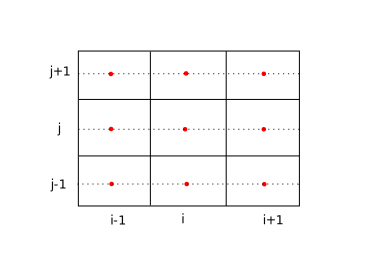
\includegraphics[width=\defaultwidth]{discrect2.pdf}
      \caption{Cartesian decomposition of the \ac{2D} domain. The dash lines represent discontinuities in the permittivity value.}
      \label{fig-decompo2}
    \end{figure}

    The discretization of the Poisson \cref{eq-poissonsum} is follows the same path as previously,except that the electric flux in equation in not constant any more, so that \cref{eq-poissonsum} becomes
    \begin{equation}
    \oint_{\C} (-\epsilon \grad \phi) \cdot \vect{n} dS = \sum_{k\in(E,W,N,S)} S^k_{i,j} <\vect{D}^k_{i,j} \cdot \vect{n}>.
    \end{equation}

    We can define
    \begin{align}
    <\vect{D}^E_{i,j} \cdot \vect{n} >&= \frac{1}{2} \epsilon_{i,j}^N E_{x, i+1/2,j}^- + \frac{1}{2} \epsilon_{i,j}^S E_{x, i+1/2,j}^-\\
     &= \frac{-1}{2} (\epsilon_{i,j}^N + \epsilon_{i,j}^S) \frac{\phi_{i+1/2,j} - \phi_{i,j}}{d_i/2}
     \label{eq-flux}
    \end{align}
    so that in the Est-West direction, the flux behave as if the cell permittivity is the mean of the North and South half plane$\epsilon_{i,j} = \frac{1}{2} (\epsilon_{i,j}^N + \epsilon_{i,j}^S)$.
    Hence, the rest of the computation is similar.
    For the boundary North and South, the permittivity is constant, hence there is no modification.
    Consequently, we obtain the discretization
    \begin{equation}
    S^E_{i,j} Q^E_{i,j} \phi_{i+1,j} + S^W_{i,j} Q^W_{i,j} \phi_{i-1,j} + S^N_{i,j} Q^N_{i,j} \phi_{i,j+1} + S^S_{i,j} Q^S_{i,j} \phi_{i,j-1} - Q^C_{i,j} \phi_{i,j} = - \V \bar{\rho_{i,j}}
    \label{eq-descretPoissoncentered}
    \end{equation}
    with
    \begin{center}
     $\begin{dcases}
     Q^E_{i,j} &= 2\frac{\epsilon_{i,j} \epsilon_{i+1,j}}{\epsilon_{i,j} d_{i+1} + \epsilon_{i+1,j} d_i} \\
     Q^W_{i,j} &= Q^E_{i-1,j} \\
     Q^N_{i,j} &= 2\frac{\epsilon_{i,j}^N \epsilon_{i,j+1}^S}{\epsilon_{i,j}^N d_{j+1} + \epsilon_{i,j+1}^S d_{j}}\\
     Q^S_{i,j} &= 2\frac{\epsilon_{i,j}^S \epsilon_{i,j-1}^N}{\epsilon_{i,j}^S d_{j+1} + \epsilon_{i,j-1}^N d_{j}} \\
     Q^C_{i,j} &= Q^E_{i,j}S^E_{i,j}+Q^W_{i,j}S^W_{i,j}+Q^N_{i,j}S^N_{i,j}+Q^S_{i,j}S^S_{i,j}
     \end{dcases}$
    \end{center}

    As well as $S^E_{i,j} = S^W_{i,j} =d_id_z, S^N_{i,j} = S^S_{i,j}= d_jd_z$ et $\V = d_jd_id_z$.
    Here, the system is no more symmetric.
    However, we can suppose that the only permittivity jump happens at the cell center, so that  $\epsilon_{i,j}^S = \epsilon_{i,j-1}^N$.
    Hence, $Q^N_{i,j} = 2\frac{\epsilon_{i,j}^N}{ d_{j+1} + d_{j}}$ and the system is symmetric.

  \subsection{Surface charges for centred interface}
    in the case of centered plasma-wall interface, we have surfaces charges at the center of the cell.
    Hence
    \begin{equation}
    \int_{\Omega_{i,j}} \rho dv = \Omega_{i,j}\bar{\rho} + S_{i,j}^N \sigma_{i,j}.
    \end{equation}
    The surface charges behave like volume charges.
    Hence, we obtain
    \begin{equation}
    S^E_{i,j} Q^E_{i,j} \phi_{i+1,j} + S^W_{i,j} Q^W_{i,j} \phi_{i-1,j} + S^N_{i,j} Q^N_{i,j} \phi_{i,j+1} + S^S_{i,j} Q^S_{i,j} \phi_{i,j-1} - Q^C_{i,j} \phi_{i,j} = - \V \bar{\rho_{i,j}} - S^N_{i,j} \sigma_{i,j}
    \end{equation}

    The discretization obtained for the plasma-wall interface cell-centred is very similar to the one obtained for the interface at the cell interface.
    However, it conserves the particle domain when the dielectric layer is not modeled and that Dirichlet conditions are applied, and the electric field at the plasma-wall interface is better defined.
    Hence, the cell-centred interface will be used.

    \inlinenote{Ajouter validation de la resolution}
    
  \subsection{Electric field computation}
  
  \subsection{Numerical resolution the Poisson equation}
  
  
% !TEX root=/home/tavant/these/manuscript/src/manuscript.tex

\section{Axial Convection model}
  \label{sec-reinjectionnoise}
  \inlinenote{Add the section about reinjection noise.}

  As introduce in the previous section, the \ac{2D} radial-azimuthal simulation do not model a priori the convection.

  \subsection{Lafleur's model of injection}

    \citet{lafleur2016a} proposed a way to model the axial convection of the particles in a \ac{1D} purely azimuthal simulation.
    \Cref{fig-Fake_1d_1} shows a schematic illustration of the model.
    The principle is as follow
    \begin{itemize}
      \item We set a finite axial length, noted $L_z$ on \cref{fig-Fake_1d_1}.
      \item We follow the positions of the particle in the axial direction $z$
      \item When a particle crosses the boundary, it is removed.
      \item A new particle is created
      \begin{itemize}
        \item at $z=0$ for the ions
        \item  at $z=L_z$ for the electrons
      \end{itemize}
    \end{itemize}

    We create a new particle in order to conserve the charge in the simulation.
    The new particle has a velocity following a Maxwellian flux distribution function of a given temperature.
    The azimuthal position of the particle is chosen uniformly at random.

    \improvement{Add definition of the Maxellian and maxellian flux VDF ?}

    \begin{figure}[hbtp]
      \centering
      \includegraphics[width=\defaultwidth]{Fake_1d_2}
      \caption{Schematic representation of Trevor's convection model \citep{lafleur2016a}. The red particle is removed of the simulation, and the green particle is created. In this illustration, the particle is an ion. }
      \label{fig-Fake_1d_1}
    \end{figure}

    Lafleur's model of convection has been adopted in \ac{2D} by \citet{croes2017a}.
    The principle is exactly similar.
    The particles are followed in the 3 directions, and a finite length is used to close to axial direction.
    It is important to note that even is the particle are followed in the 3 directions, the meshed domain is only \ac{2D}.
    The simulation is not \ac{3D}-\ac{3V}.

    In \citet{croes2017a}, the authors have observed that if the newly created particle has a radial position chosen uniformly at random, it would affect the sheath.
    Hence, they decided to use the same radial position that the removed particle.
    \Cref{fig-Fake_2d} presents a schematic representation of the convection model in \ac{2D}.

    \begin{figure}[hbtp]
      \centering
      \includegraphics[width=\defaultwidth]{2_5D_dielectric_PPS_small}
      \caption{Schematic representation of the Lafleur's convection model adapted in \ac{2D}. The new particle radial position corresponds to the removed particle, but its azimuthal position is chosen uniformly at random. }
      \label{fig-Fake_2d}
    \end{figure}

    \Cref{fig-energy_convection} shows the evolution as a function of time of the electron mean energy in the simulation in a typical \ac{2D} radial-azimuthal simulation, addapted from \citet{croes2017}.
    We can see that without the convection, the mean energy quickly rises to unphysical values.
    When the convection is modeled, using an axial of $L_z=1$ cm, the energy reaches a steady state.
    \nomenclature[Q]{\ensuremath{ L_z}}{ Axial length}
    \begin{figure}[hbtp]
      \centering
      \includegraphics[width=\defaultwidth]{energy}
      \caption{Time evolution of the electron mean energy when the convection is not modeled ($L_z \rightarrow \infty$) and with Trevor's convection model used, $L_z = 1$ cm. Adapted from \citet{croes2017}.}
      \label{fig-energy_convection}
    \end{figure}



  \subsection{Numerical artefacts}
    \citet{lafleur2016a} studied the impact of the convection model on the simulation results.
    The authors observed in particular that changing the azimuthal length of the simulation domain could affect the simulation results.

    \Cref{fig-convection_numerical} shows the time evolution of the azimuthal electric field $E_{\theta}$ from the \ac{1D} simulation \citep{lafleur2016a}.
    \nomenclature[Q]{\ensuremath{ E_{\theta}}}{ Azimuthal electric field}

    On the first row (\cref{fig-convection_numerical}.{\bf a} and {\bf b}), the length of the periodic azimuthal direction is $L_{\theta}=0.5$~cm.
    \cref{fig-convection_numerical}.{\bf a} corresponds to the case without axial convection.
    We clearly see that the \ac{ECDI} rises and do not saturate.
    The wavelength is short, of the order of $\lambda = 1.5$~mm.
    \nomenclature[Q]{\ensuremath{ \lambda}}{ Wave length}
    \cref{fig-convection_numerical}.{\bf b} corresponds to the same case as \cref{fig-convection_numerical}.{\bf a} but this time with the axial convection modeled.
    We observe this time a saturation of the oscillation's amplitude, and the wavelength is close to $\lambda = 1.5$~mm.

    On the second row (\cref{fig-convection_numerical}.{\bf c} and {\bf d}), the length of the periodic azimuthal direction is $L_{\theta}=1$~cm.
    \cref{fig-convection_numerical}.{\bf c} corresponds to the case without axial convection, and \cref{fig-convection_numerical}.{\bf b} corresponds to the same case but this time with the axial convection modeled.
    In \cref{fig-convection_numerical}.{\bf c}, we can see that increasing the azimuthal length did not affect the \ac{ECDI}, as expected.
    However, in  \cref{fig-convection_numerical}.{\bf d}, the instability is clearly affected.
    A simple oscillation is observe, corresponding to $\lambda=10$~mm.
    They are most certainly unphysical.

    \begin{figure}[hbtp]
      \centering

      \begin{tabular}{cc}
        \subfigure{Lafleur_NoLz_1}{a}{20, 20}
            &
        \subfigure{Lafleur_Lz_1}{b}{20, 20} \\

        \subfigure{Lafleur_NoLz_2}{c}{20, 20} &
        \subfigure{Lafleur_Lz_2}{d}{20, 20} \\
      \end{tabular}
      \caption{Effects of Lafleur's convection model for two different azimuthal length on the azimuthal electric field. ({\bf a}) No convection, $L_x=0.5$~cm,  ({\bf b}) convection modeled, $L_x=0.5$~cm,  ({\bf c}) No convection, $L_x=1$~cm,  ({\bf d}) convection modeled, $L_x=1$~cm. The colour of each plots is normalized to the maximum amplitude. Adapted from \citep{lafleur2016a}. \inlinenote{Get $\theta$ back to $y$ instead of $x$}}
      \label{fig-convection_numerical}
    \end{figure}

    \FloatBarrier
    \citet{croes2017} observed similar behaviour with the bidimensional  simulation.
    The author investigated the values of the azimuthal length which presented physical and unphysical results
    for different values of the axial length.
    \Cref{fig-couplesCroes} shows the results obtained (adapted from \citep{croes2017}).
    We can see that for a given value of the axial length, the azimuthal must be lower that a certain value to present physical results.
    However, the value of this upper limit depends of the axial length, such that the if the axial length decreases, the upper limit of the azimuthal length decreases as well.

    \begin{figure}[hbtp]
      \centering
      \includegraphics[width=\defaultwidth]{2D_couples}
      \caption{Values of the azimuthal length and the axial length for which the simulation result is physical (similar to \cref{fig-convection_numerical}.{\bf b}) or unphysical  (similar to \cref{fig-convection_numerical}.{\bf d}) \inlinenote{Make this image smaller (smaller font, etc.)}}
      \label{fig-couplesCroes}
    \end{figure}

    No explanation have been proposed, yet.
    In the next section, we develop a possible explanation, and a new convection model for the simulation.

  \subsection{Numerical noise of Lafleur's convection model}

    Let us consider de Lafleur's convection model in \ac{1D} on the charge density.
    When computing the charge density on the mesh vertices, the axial position is not taken into account.
    Consequently, the convection process illustrated on \cref{fig-Fake_1d_1} is similar to moving a particle arbitrarily.
    Seen by the charge density, this is similar to a Poisson noise, also named shot noise, on the charge density.
    \inlinenote{Actually, this is more like the combination of a Poisson noise with a uniform noise, appending twice for every particles, once with a positive charge and once with a negative charge. I don't really know if we need to give these details. }

    After a certain number of particle removed and created, the Poisson noise is similar to a Gaussian noise, also named thermal noise, following a normal distribution $\N$ .
    \nomenclature[Q]{\ensuremath{ \N }}{ Normal distribution.}
    Hence, the charge density becomes
    \begin{equation} \label{eq-rhonoise}
      \rho = \rho_0 + \N(0, \stdconv),
    \end{equation}
    with $\rho$ the charge density, $\rho_0$ the charge density without the convection process, and $\stdconv$ the standard deviation of the distribution of the noise associated with the convection model.
    \nomenclature[Q]{\ensuremath{ \rho}}{ Charge density}
    \nomenclature[Q]{\ensuremath{ \stdconv}}{ tandard deviation of the distribution of the noise associated with the convection model}
    Surprisingly, the noise due to the convection model is similar to the numerical noise induced by the decomposition of the plasma into particles $\N(0, \sigma_{\rm stat})$.
    However, the amplitude of this statistical noise decreases with the number of particles per cell used
    \begin{equation*} \label{eq-statistical}
     \sigma_{\rm stat} \propto \frac{1}{\sqrt{N_{pc}}}.
    \end{equation*}

    On the other hand, the amplitude of the noise induced by the convection model depends on the plasma density $n$, the axis velocity of the particles $v_z$ and the axial length $L_z$
    \begin{equation} \label{eq-convstd}
     \stdconv \propto \frac{n}{L_z} v_z.
    \end{equation}

    We can see on \cref{eq-convstd} that the amplitude of the convection induced noise on the charge density is proportional to the inverse of the axial length $L_z$.
    This could explain the observation of \cref{fig-couplesCroes} that obtaining physical result with a smaller $L_z$ is more restrictive.
    However, it do not explain the effects of the azimuthal length.

  \subsection{Effect of the noise on the electric field}

% !TEX root=/home/tavant/these/manuscript/src/manuscript.tex

\section{Electron induced secondary electron emission from the wall}
\label{sec-seemodel}
When an incident electron reaches the wall material, several scenarii are possible, as described in \citet{villemant2018}
\begin{enumerate}
  \item Elastic reflection\string: the electron encounters only elastic collision with the material, hence its energy is constant. However, its reflection is not necessary specular.
  \item Inelastic reflection\string: the electron looses some of its energy to the material before returning to the plasma.
  \item Secondary electron emission\string: the energy of the primary electron is enough to extract one or more electrons from the material.
  \item No emission, the electron is absorbed by the wall.
\end{enumerate}

The probability \proba{}  that one event happens instead of another depends predominantly on the particle energy, and weakly on its  impact angle.
Concerning the mean flux of electron incident and emitted, we uses the mean emission rate, or yield, \rate
\begin{equation*} \label{eq-ratedifinition}
  \rate = \frac{\Gamma_{e, \rm secondary}}{\Gamma_{e, \rm primary}}
\end{equation*}
which can be developed using the distribution function to 
\begin{equation*} \label{eq-ratedifinition_evdf}
  \rate = \frac{\iiint_{\Omega} v_x \proba(\vect{v_e}) f(\vect{v_e}) d^3v}{\iiint_{\Omega} v_x \proba(\vect{v_e}) f(\vect{v_e}) d^3v}
\end{equation*}
with $\Omega$ the ensemble of $\vect{v_e}$ directed toward the wall\string: $\vect{v_e} \cdot \vect{n} > 0$, with $\vect{n} $ the unit vector normal to and toward the wall.

\subsection{Models of emission } \label{subsec-seemodels}
Several models can be used to describe the electron emission.

\paragraph{Monte Carlo models} are the more realistic.
 They are based on the computation of the trajectory of the electrons through the material, during which the electron can encounter several interactions with the material.
 Each interactions can modify the electron direction, energy, and generate new electron.
 Several models have been proposed, as \citet{furman2002,pierron2017}.
 These models allow a precise characterization of the processes, but depends on a large number of parameters difficult to obtain due to the lack of experimental data.
 
\paragraph{Analytical models} provides a simplified description of the rate of emission.
Their complexity depends on the precision desired.
The most largely used are the models of \citet{vaughan1989,barral2003a,sydorenko2006b}.

In this work, we are interested only in representing qualitatively the electron emission.
Moreover, \citet{croes2017} showed that changing the model used do not affect significantly the results. 
Hence, we will use the model of \citet{barral2003a} for its simplicity.

\subsection{Barral electron emission model}
\label{sec-modelused}

The emission model used follows a linear-saturated law for the probability of emission with three parameters. 
It describes the total emission corresponding to the sum of the elastic and inelastic backscattering and the secondary electron emission.
\begin{equation} \label{eq-proba_barral}
  \proba(\ek) = 
  \begin{cases}
    \proba_0 + (1 - \proba_0) \frac{\ek}{\crover}   &\text{ if } \ek <  \ek_{\max} \\
    \probamax &\text{ if } \ek \geq \ek_{\max}
  \end{cases}
\end{equation}
where $\ek$ is the kinetic energy of the incoming electron, $\proba_0$ is the asymptotic probability of emission at energy null, $\crover$ is the crossover energy above which the probability of emission is higher that one, \probamax is the maximum probability and $\ek_{\max}= \frac{\probamax - \proba_0}{1 - \proba_0} \crover $ is the minimum energy for which $\rate = \probamax$.
\Cref{eq-proba_barral} is illustrated in \Cref{fig-modelbarral}.

\begin{figure}[hbtp]
  \centering
  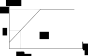
\includegraphics[width=\defaultwidth]{barral}
  \caption{Linear-saturated emission model from \citet{barral2003a}.}
  \label{fig-modelbarral}
\end{figure}

 We suppose that all of the electrons emitted are isotropically emitted following a Maxwellian flux distribution function of temperature $\Tsee$.
 The parameters $\proba_0$,  $\probamax$ and $\crover$ can be obtained from experiments. 
 \Cref{tab-seeparames} shows the crossover energy and the  probability of emission at energy null for different materials.
 The value of $\proba_0$ is always close to $0.5$, but $\crover$ can vary from 18 to 305 V.
 Hence, in the following parametric studies, $\proba_0$ will be kept at 0.5 while we vary $\crover$ from low values, corresponding to highly emmissive materials, to high values, representing less emmissive materials.
 
 \begin{table}[hbtp]
   \ra{1.3}
   \centering
   \caption{Emission parameters for different materials, from \citet{barral2003a}.}
   \label{tab-seeparames}
   \begin{tabular}{@{}lll@{}} \toprule
   Material & $\crover$ (V)& $\proba_0$ \\ \midrule
   BN-SiO$_2$ & 53 & 0.45 \\ 
   Al$_2$O$_3$ & 18  & 0.57 \\ 
   SiC     &  43  &0.69  \\
   Graphite & 305  & 0.40 \\ 
   \bottomrule
   \end{tabular}
 \end{table}
 
 Since the model used describe both the reflected and true secondary electron emission, we will use the general name \emph{electron emission}  to refer to the flux of electron comming from the wall toward the plasma.
 In contrast, the electrons reaching the plasma are referred to as the \emph{primary electrons}.

% !TEX root=/home/tavant/these/manuscript/src/manuscript.tex

\section{Study of electron cross field transport with a 2D radial-azimuthal PIC simulation}
  \label{sec-transport}
  
  \inlinenote{Rq de Anne: Mettre cette section sur la mobilite dans Chapter 0. Reponse: Ok, peut etre pas toutes les formules...? }
  \inlinenote{Anne: Revoir la transition, et mettre ici que les calcules numerique. L'état de l'art peut être ajouter au ch 0.}
  \inlinenote{Anne: transition ici à revoir....c'est un peu brutal : jusqu'ici on te suit car tu pars d'une description generale du PIC pour parler plus en detail des parois (Poisson, emission secondaire, gaine...)
Je pense que la premiere phrase de la 1.8 pourrait etre un truc du genre...
A key topic of my PhD work is to study the impact of surface processes on the plasma discharge and in particular on the electron mobility. }
  
  \inlinenote{Anne: je mettrai une grande partie du texte de cette page dans le chapitre 0 et je rappellerai ici juste les expressions de mu eff, mu classic, mu sat...et dire en 2 phrases comment ils sont calculés en PIC.}
  
  The electron mobility in the axial direction $\mobe$ is defined as the ratio between the mean velocity $u$ and the electric field
  \begin{equation} \label{eq-mudef}
    \mobe = \frac{u_{e,z}}{E_z}
  \end{equation}
  with $u_{e,z}=<v_{e,z}>$ the electron mean velocity.
  \nomenclature[Q]{\ensuremath{ u_{e,z}}}{Electron mean velocity in the axial direction\string: $u_{e,z} = < v_{e,z}>$}
  In the \ac{PIC} simulations, \cref{eq-mudef} can be used directly to compute $\mobpic$.
  
  In the classical drift diffusion theory of the electron mobility transverse to a magnetic field, the mobility is due to collisions as seen in \cref{eq-mobility} 
  \begin{equation} \label{eq-mobclas}
    \mobcla = \frac{e}{m_e} \frac{\nu_m}{\nu_m^2 + \oce^2}
  \end{equation}
  with $\oce=\frac{e B}{m_e}$ the electron cyclotron frequency and $\nu_m$ the electron-neutral momentum transfer collision frequency.
  \nomenclature[Q]{\ensuremath{ \oce}}{ Electron cyclotron frequency $\oce=\frac{e B}{m_e}$}
  \nomenclature[Q]{\ensuremath{ \nu_m}}{  electron-neutral momentum transfer collision frequency}
  
  At the exit plane, the classical mobility predicts a mobility of the order of $\mobcla=0.001-0.01\mobunit$ \citep{adam2008a}.
  
  The kinetic approach allowed \citet{lafleur2016a} to propose a modified mobility due to the oscillations of the electron density and the azimuthal electric field of the \ac{ECDI}.
  This effective mobility obtained is 
  \begin{equation} \label{eq-defmobeff}
    \mobeff = \mobcla \lp 1 - \frac{\oce}{\nu_m}  \frac{< \dne \dEt >_{\theta} }{n_0 E_z}   \rp
  \end{equation}
  with \dne{} and \dEt{} the fluctuations in the azimuthal directions of the electron density and azimuthal electric field, respectively, the operator $< . >_{\theta}$ is the average in the azimuthal direction, and $n_0$ is the average plasma density.
  In the case where $\nu_m << \oce$, \cref{eq-defmobeff} can be simplified to 
  \begin{align} 
    \mobeff &= \frac{\frac{e}{m_e} \nu_m}{\oce^2} \lp 1 - \frac{\oce^2}{\nu_m}  \frac{< \dne \dEt >_{\theta} }{n_0 E_z}   \rp \nonumber \\
    &= \frac{< \dne \dEt >_{\theta} }{n_0 E_z}   \frac{1}{B_r} \label{eq-mobeffsimple}
  \end{align}
  which shows that the instability enhances the electron axial mobility in a wave similar to an $E \times B$ drift.
  The electric field $E_{\theta}$ oscillates and presents a zero mean value, but the average effect on the electron transport is not zero if the correction between \dEt{} and \dne{} is not zero.
  
  In  \citet{lafleur2016a}, the authors present the instability effect as an electron-ion friction force $\Rei = - e < \dne \dEt >_{\theta}$.
  Under the assumption that the saturation of the instability is mainly due to ion trapping, the electron-ion friction force can be simplified in the \ac{2D} geometry of the simulation to
  \begin{equation} \label{eq-rei-sat}
    \Rei^{sat} = \frac{e \norm{\grad \cdot (n_e \Te \vect{v_i})}}{4 \sqrt{6} c_s} \simeq \frac{e n_e \Te \viout}{4 \sqrt 6 c_s L_z}
  \end{equation} 
  \nomenclature[Q]{\ensuremath{ \vect{v_i}}}{  ion velocity vector}
  \nomenclature[Q]{\ensuremath{ c_s}}{ ion sound speed $c_s=(e \Te/m_i)^{1/2}$ }
  where $\vect{v_i}$ is the ion velocity, $c_s=(e \Te/m_i)^{1/2}$  is the ion sound speed, and the spatial derivative in has been approximated across the axial simulation direction, with $\viout$ the ion outlet velocity 
  \begin{equation} \label{eq-viz}
    \viout = \sqrt{\frac{2 e U_z}{m_i}},
  \end{equation}
  with $U_z = E_z L_z$ the total potential difference in the axial direction.
  \nomenclature[Q]{\ensuremath{ U_z}}{   total potential difference in the axial direction $U_z = E_z L_z$}
  
  Using \cref{eq-rei-sat} in \cref{eq-mobeffsimple}, we obtain the simplified expression of the effective mobility at saturation
  \begin{equation} \label{eq-mobeffsat}
    \mobeffsat = \frac{\sqrt{\frac{\Te}{U_z}}}{4\sqrt{3}B_r}.
  \end{equation}
  
  \Cref{eq-mobeffsat} shows that for the radial and azimuthal \ac{2D} geometry being used here, the enhanced mobility due to \ac{ECDI} scales as the square-root of the electron temperature $\Te$ if the simulation parameters are constant.
  However, it is not the case in general, as the saturation of the instability can be also due to convection, and there are axial gradients in the electron temperature and plasma density as well.
  
  We can note that $\mobpic, \mobeff$ and $\mobcla$ are defined at every position of the simulation, but that $\mobeffsat$ can only be globally calculated. 
  
  
  
  
  
% !TEX root=/home/tavant/these/manuscript/src/manuscript.tex



\section{Conclusion}
  \label{sec-conclusion_ch1}
  
  In order to study the plasma wall interaction in an \ac{HET}, we developed a bi-dimensional simulation code using \ac{PIC}-\ac{MCC} modeling.
  As the electrons drift azimuthally due to the $E \times B$ configuration, the \ac{ECDI} rises, enhancing the cross field transport of the electron toward the anode.
  The walls closing the chamber in the radial direction are also important for the discharge behaviour.
  Hence, in order to compare the interaction between these phenomena, we simulate the radial-azimuthal domain.
  
  A special care have been taken concerning
  \begin{itemize}
    \item the modeling of the axial convection, in order to model the energy losses and so attain a steady state,
    \item the modeling of the radial boundary with the dielectric layer included in the simulation domain.
  \end{itemize}
  
  \inlinenote{Add a {\it typical result} to describe the may behaviour of the simulation ?}
  
  
